% Options for packages loaded elsewhere
% Options for packages loaded elsewhere
\PassOptionsToPackage{unicode}{hyperref}
\PassOptionsToPackage{hyphens}{url}
\PassOptionsToPackage{dvipsnames,svgnames,x11names}{xcolor}
%
\documentclass[
  american,
  letterpaper,
  DIV=11,
  numbers=noendperiod]{scrartcl}
\usepackage{xcolor}
\usepackage{amsmath,amssymb}
\setcounter{secnumdepth}{5}
\usepackage{iftex}
\ifPDFTeX
  \usepackage[T1]{fontenc}
  \usepackage[utf8]{inputenc}
  \usepackage{textcomp} % provide euro and other symbols
\else % if luatex or xetex
  \usepackage{unicode-math} % this also loads fontspec
  \defaultfontfeatures{Scale=MatchLowercase}
  \defaultfontfeatures[\rmfamily]{Ligatures=TeX,Scale=1}
\fi
\usepackage{lmodern}
\ifPDFTeX\else
  % xetex/luatex font selection
\fi
% Use upquote if available, for straight quotes in verbatim environments
\IfFileExists{upquote.sty}{\usepackage{upquote}}{}
\IfFileExists{microtype.sty}{% use microtype if available
  \usepackage[]{microtype}
  \UseMicrotypeSet[protrusion]{basicmath} % disable protrusion for tt fonts
}{}
\makeatletter
\@ifundefined{KOMAClassName}{% if non-KOMA class
  \IfFileExists{parskip.sty}{%
    \usepackage{parskip}
  }{% else
    \setlength{\parindent}{0pt}
    \setlength{\parskip}{6pt plus 2pt minus 1pt}}
}{% if KOMA class
  \KOMAoptions{parskip=half}}
\makeatother
% Make \paragraph and \subparagraph free-standing
\makeatletter
\ifx\paragraph\undefined\else
  \let\oldparagraph\paragraph
  \renewcommand{\paragraph}{
    \@ifstar
      \xxxParagraphStar
      \xxxParagraphNoStar
  }
  \newcommand{\xxxParagraphStar}[1]{\oldparagraph*{#1}\mbox{}}
  \newcommand{\xxxParagraphNoStar}[1]{\oldparagraph{#1}\mbox{}}
\fi
\ifx\subparagraph\undefined\else
  \let\oldsubparagraph\subparagraph
  \renewcommand{\subparagraph}{
    \@ifstar
      \xxxSubParagraphStar
      \xxxSubParagraphNoStar
  }
  \newcommand{\xxxSubParagraphStar}[1]{\oldsubparagraph*{#1}\mbox{}}
  \newcommand{\xxxSubParagraphNoStar}[1]{\oldsubparagraph{#1}\mbox{}}
\fi
\makeatother

\usepackage{color}
\usepackage{fancyvrb}
\newcommand{\VerbBar}{|}
\newcommand{\VERB}{\Verb[commandchars=\\\{\}]}
\DefineVerbatimEnvironment{Highlighting}{Verbatim}{commandchars=\\\{\}}
% Add ',fontsize=\small' for more characters per line
\newenvironment{Shaded}{}{}
\newcommand{\AlertTok}[1]{\textcolor[rgb]{1.00,0.00,0.00}{\textbf{#1}}}
\newcommand{\AnnotationTok}[1]{\textcolor[rgb]{0.38,0.63,0.69}{\textbf{\textit{#1}}}}
\newcommand{\AttributeTok}[1]{\textcolor[rgb]{0.49,0.56,0.16}{#1}}
\newcommand{\BaseNTok}[1]{\textcolor[rgb]{0.25,0.63,0.44}{#1}}
\newcommand{\BuiltInTok}[1]{\textcolor[rgb]{0.00,0.50,0.00}{#1}}
\newcommand{\CharTok}[1]{\textcolor[rgb]{0.25,0.44,0.63}{#1}}
\newcommand{\CommentTok}[1]{\textcolor[rgb]{0.38,0.63,0.69}{\textit{#1}}}
\newcommand{\CommentVarTok}[1]{\textcolor[rgb]{0.38,0.63,0.69}{\textbf{\textit{#1}}}}
\newcommand{\ConstantTok}[1]{\textcolor[rgb]{0.53,0.00,0.00}{#1}}
\newcommand{\ControlFlowTok}[1]{\textcolor[rgb]{0.00,0.44,0.13}{\textbf{#1}}}
\newcommand{\DataTypeTok}[1]{\textcolor[rgb]{0.56,0.13,0.00}{#1}}
\newcommand{\DecValTok}[1]{\textcolor[rgb]{0.25,0.63,0.44}{#1}}
\newcommand{\DocumentationTok}[1]{\textcolor[rgb]{0.73,0.13,0.13}{\textit{#1}}}
\newcommand{\ErrorTok}[1]{\textcolor[rgb]{1.00,0.00,0.00}{\textbf{#1}}}
\newcommand{\ExtensionTok}[1]{#1}
\newcommand{\FloatTok}[1]{\textcolor[rgb]{0.25,0.63,0.44}{#1}}
\newcommand{\FunctionTok}[1]{\textcolor[rgb]{0.02,0.16,0.49}{#1}}
\newcommand{\ImportTok}[1]{\textcolor[rgb]{0.00,0.50,0.00}{\textbf{#1}}}
\newcommand{\InformationTok}[1]{\textcolor[rgb]{0.38,0.63,0.69}{\textbf{\textit{#1}}}}
\newcommand{\KeywordTok}[1]{\textcolor[rgb]{0.00,0.44,0.13}{\textbf{#1}}}
\newcommand{\NormalTok}[1]{#1}
\newcommand{\OperatorTok}[1]{\textcolor[rgb]{0.40,0.40,0.40}{#1}}
\newcommand{\OtherTok}[1]{\textcolor[rgb]{0.00,0.44,0.13}{#1}}
\newcommand{\PreprocessorTok}[1]{\textcolor[rgb]{0.74,0.48,0.00}{#1}}
\newcommand{\RegionMarkerTok}[1]{#1}
\newcommand{\SpecialCharTok}[1]{\textcolor[rgb]{0.25,0.44,0.63}{#1}}
\newcommand{\SpecialStringTok}[1]{\textcolor[rgb]{0.73,0.40,0.53}{#1}}
\newcommand{\StringTok}[1]{\textcolor[rgb]{0.25,0.44,0.63}{#1}}
\newcommand{\VariableTok}[1]{\textcolor[rgb]{0.10,0.09,0.49}{#1}}
\newcommand{\VerbatimStringTok}[1]{\textcolor[rgb]{0.25,0.44,0.63}{#1}}
\newcommand{\WarningTok}[1]{\textcolor[rgb]{0.38,0.63,0.69}{\textbf{\textit{#1}}}}

\usepackage{longtable,booktabs,array}
\usepackage{calc} % for calculating minipage widths
% Correct order of tables after \paragraph or \subparagraph
\usepackage{etoolbox}
\makeatletter
\patchcmd\longtable{\par}{\if@noskipsec\mbox{}\fi\par}{}{}
\makeatother
% Allow footnotes in longtable head/foot
\IfFileExists{footnotehyper.sty}{\usepackage{footnotehyper}}{\usepackage{footnote}}
\makesavenoteenv{longtable}
\usepackage{graphicx}
\makeatletter
\newsavebox\pandoc@box
\newcommand*\pandocbounded[1]{% scales image to fit in text height/width
  \sbox\pandoc@box{#1}%
  \Gscale@div\@tempa{\textheight}{\dimexpr\ht\pandoc@box+\dp\pandoc@box\relax}%
  \Gscale@div\@tempb{\linewidth}{\wd\pandoc@box}%
  \ifdim\@tempb\p@<\@tempa\p@\let\@tempa\@tempb\fi% select the smaller of both
  \ifdim\@tempa\p@<\p@\scalebox{\@tempa}{\usebox\pandoc@box}%
  \else\usebox{\pandoc@box}%
  \fi%
}
% Set default figure placement to htbp
\def\fps@figure{htbp}
\makeatother


% definitions for citeproc citations
\NewDocumentCommand\citeproctext{}{}
\NewDocumentCommand\citeproc{mm}{%
  \begingroup\def\citeproctext{#2}\cite{#1}\endgroup}
\makeatletter
 % allow citations to break across lines
 \let\@cite@ofmt\@firstofone
 % avoid brackets around text for \cite:
 \def\@biblabel#1{}
 \def\@cite#1#2{{#1\if@tempswa , #2\fi}}
\makeatother
\newlength{\cslhangindent}
\setlength{\cslhangindent}{1.5em}
\newlength{\csllabelwidth}
\setlength{\csllabelwidth}{3em}
\newenvironment{CSLReferences}[2] % #1 hanging-indent, #2 entry-spacing
 {\begin{list}{}{%
  \setlength{\itemindent}{0pt}
  \setlength{\leftmargin}{0pt}
  \setlength{\parsep}{0pt}
  % turn on hanging indent if param 1 is 1
  \ifodd #1
   \setlength{\leftmargin}{\cslhangindent}
   \setlength{\itemindent}{-1\cslhangindent}
  \fi
  % set entry spacing
  \setlength{\itemsep}{#2\baselineskip}}}
 {\end{list}}
\usepackage{calc}
\newcommand{\CSLBlock}[1]{\hfill\break\parbox[t]{\linewidth}{\strut\ignorespaces#1\strut}}
\newcommand{\CSLLeftMargin}[1]{\parbox[t]{\csllabelwidth}{\strut#1\strut}}
\newcommand{\CSLRightInline}[1]{\parbox[t]{\linewidth - \csllabelwidth}{\strut#1\strut}}
\newcommand{\CSLIndent}[1]{\hspace{\cslhangindent}#1}

\ifLuaTeX
\usepackage[bidi=basic]{babel}
\else
\usepackage[bidi=default]{babel}
\fi
% get rid of language-specific shorthands (see #6817):
\let\LanguageShortHands\languageshorthands
\def\languageshorthands#1{}
\ifLuaTeX
  \usepackage[english]{selnolig} % disable illegal ligatures
\fi


\setlength{\emergencystretch}{3em} % prevent overfull lines

\providecommand{\tightlist}{%
  \setlength{\itemsep}{0pt}\setlength{\parskip}{0pt}}



 


\KOMAoption{captions}{tableheading}
\makeatletter
\@ifpackageloaded{tcolorbox}{}{\usepackage[skins,breakable]{tcolorbox}}
\@ifpackageloaded{fontawesome5}{}{\usepackage{fontawesome5}}
\definecolor{quarto-callout-color}{HTML}{909090}
\definecolor{quarto-callout-note-color}{HTML}{0758E5}
\definecolor{quarto-callout-important-color}{HTML}{CC1914}
\definecolor{quarto-callout-warning-color}{HTML}{EB9113}
\definecolor{quarto-callout-tip-color}{HTML}{00A047}
\definecolor{quarto-callout-caution-color}{HTML}{FC5300}
\definecolor{quarto-callout-color-frame}{HTML}{acacac}
\definecolor{quarto-callout-note-color-frame}{HTML}{4582ec}
\definecolor{quarto-callout-important-color-frame}{HTML}{d9534f}
\definecolor{quarto-callout-warning-color-frame}{HTML}{f0ad4e}
\definecolor{quarto-callout-tip-color-frame}{HTML}{02b875}
\definecolor{quarto-callout-caution-color-frame}{HTML}{fd7e14}
\makeatother
\makeatletter
\@ifpackageloaded{caption}{}{\usepackage{caption}}
\AtBeginDocument{%
\ifdefined\contentsname
  \renewcommand*\contentsname{Table of contents}
\else
  \newcommand\contentsname{Table of contents}
\fi
\ifdefined\listfigurename
  \renewcommand*\listfigurename{List of Figures}
\else
  \newcommand\listfigurename{List of Figures}
\fi
\ifdefined\listtablename
  \renewcommand*\listtablename{List of Tables}
\else
  \newcommand\listtablename{List of Tables}
\fi
\ifdefined\figurename
  \renewcommand*\figurename{Figure}
\else
  \newcommand\figurename{Figure}
\fi
\ifdefined\tablename
  \renewcommand*\tablename{Table}
\else
  \newcommand\tablename{Table}
\fi
}
\@ifpackageloaded{float}{}{\usepackage{float}}
\floatstyle{ruled}
\@ifundefined{c@chapter}{\newfloat{codelisting}{h}{lop}}{\newfloat{codelisting}{h}{lop}[chapter]}
\floatname{codelisting}{Listing}
\newcommand*\listoflistings{\listof{codelisting}{List of Listings}}
\makeatother
\makeatletter
\makeatother
\makeatletter
\@ifpackageloaded{caption}{}{\usepackage{caption}}
\@ifpackageloaded{subcaption}{}{\usepackage{subcaption}}
\makeatother
\usepackage{bookmark}
\IfFileExists{xurl.sty}{\usepackage{xurl}}{} % add URL line breaks if available
\urlstyle{same}
\hypersetup{
  pdftitle={PADRÕES DE ESTRUTURA E DIVERSIDADE DA COMUNIDADE ZOOPLANCTÔNICA EM UM AMBIENTE AQUÁTICO TEMPORÁRIO DO SEMIÁRIDO BRASILEIRO},
  pdfauthor={Steve Purves; Rowan Cockett},
  pdflang={en-US},
  pdfkeywords={La Palma, Earthquakes},
  colorlinks=true,
  linkcolor={blue},
  filecolor={Maroon},
  citecolor={Blue},
  urlcolor={Blue},
  pdfcreator={LaTeX via pandoc}}


\title{PADRÕES DE ESTRUTURA E DIVERSIDADE DA COMUNIDADE ZOOPLANCTÔNICA
EM UM AMBIENTE AQUÁTICO TEMPORÁRIO DO SEMIÁRIDO BRASILEIRO}
\usepackage{etoolbox}
\makeatletter
\providecommand{\subtitle}[1]{% add subtitle to \maketitle
  \apptocmd{\@title}{\par {\large #1 \par}}{}{}
}
\makeatother
\subtitle{Subtitle 1 Subtitle 2}
\author{Steve Purves \and Rowan Cockett}
\date{2026-04-29}
\begin{document}
\maketitle
\begin{abstract}
Abstract
\end{abstract}

\renewcommand*\contentsname{Table of contents}
{
\hypersetup{linkcolor=}
\setcounter{tocdepth}{3}
\tableofcontents
}
\listoffigures
\listoftables

\section{Introduction}\label{introduction}

O semiárido brasileiro é caracterizado por clima quente e seco, com
regime pluviométrico irregular e concentrado em poucos meses do ano,
resultando em longos períodos de estiagem, intercalados por eventos de
chuva intensa (IPBES, 2019; Ramos \emph{et al}., 2023). Essa
variabilidade climática exerce forte influência sobre a dinâmica dos
ecossistemas aquáticos da região, tornando o regime hidrológico um dos
principais fatores estruturantes da biodiversidade local. Nesse
contexto, os corpos d'água temporários assumem papel central na
manutenção da diversidade biológica, uma vez que funcionam como
ambientes de abrigo, reprodução e alimentação, garantindo a
sobrevivência de comunidades especializadas e adaptadas às flutuações
ambientais sazonais (Medeiros \emph{et al.}, 2008; Melo \& Medeiros,
2013).

As lagoas temporárias são ecossistemas aquáticos caracterizados por
ciclos hidrológicos alternados entre períodos de inundação e dessecação,
apresentando elevada heterogeneidade espacial e temporal (Medeiros
\emph{et al}., 2008; Brendonck \emph{et al}., 2021). Esses ambientes
são, em geral, rasos, de pequena extensão e isolados de fontes
permanentes de água, sendo fortemente influenciados pela dinâmica
climática local e pelo regime de chuvas (Coccia \emph{et al}., 2024).
Essas lagoas respondem rapidamente às variações climáticas,
especialmente ao regime pluviométrico, o que resulta em mudanças
contínuas na estrutura do habitat (Melo e Medeiros, 2013; Ramos \emph{et
al}., 2023).

Durante o período chuvoso, o aumento do volume hídrico provoca
modificações na morfologia das lagoas e intensifica o aporte de
nutrientes por escoamento superficial, alterando parâmetros
físico-químicos como pH, condutividade elétrica, turbidez e oxigênio
dissolvido, fenômeno observado em estudos sobre a variação
espaço-temporal de parâmetros limnológicos em ambientes aquáticos
tropicais (Rodrigues; Chagas Silva; Nascimento Barreto, 2024; Coccia
\emph{et al}., 2024). em contraste, no período seco ocorre a redução
progressiva do volume hídrico, levando à fragmentação dos habitats
aquáticos e à intensificação de condições ambientais extremas, como o
aumento da temperatura e da salinidade, além da diminuição da
disponibilidade de oxigênio (Melo e Medeiros, 2013; Brendonck \emph{et
al.}, 2021). Essas variações atuam como filtros ambientais, selecionando
espécies com características funcionais compatíveis com cada fase do
ciclo hidrológico e capazes de se estabelecer na comunidade (Kraft
\emph{et al}., 2015).

Os organismos que habitam lagoas temporárias desenvolveram estratégias
adaptativas específicas para sobreviver às variações impostas pelo ciclo
hidrológico irregular, como a produção de estágios de resistência, a
entrada em diapausa durante a fase seca e a rápida colonização após o
reenchimento (Medeiros \& Maltchik, 2001; Brendonck \emph{et al.},
2021). Além disso, a presença de bancos de propágulos no sedimento
desempenha papel fundamental na regeneração das comunidades aquáticas,
garantindo a reocupação do habitat após eventos de seca prolongada
(Frisch \emph{et al.}, 2014).

O zooplâncton, composto principalmente por Rotifera, Cladocera e
Copepoda, desempenha papel fundamental na dinâmica dos ecossistemas
aquáticos, atuando na ciclagem de nutrientes, no fluxo de energia e como
elo entre produtores primários e níveis tróficos superiores (Tundisi e
Tundisi, 2008; Souza \emph{et al}., 2025). Devido ao curto ciclo de vida
e à elevada sensibilidade às variações ambientais, esses organismos
respondem rapidamente às mudanças nas condições físico-químicas e
hidrológicas, sendo amplamente utilizados como bioindicadores da
dinâmica ecológica dos sistemas aquáticos (Vieira \emph{et al}., 2009;
Melo \& Medeiros, 2013).

A diversidade taxonômica e funcional do zooplâncton é determinada, em
grande medida, pela extensão do hidroperíodo, sendo mais elevada em
lagoas com maior tempo de permanência da água, enquanto ambientes com
ciclos hidrológicos mais curtos tendem a apresentar comunidades mais
simplificadas e dominadas por espécies oportunistas (Vanschoenwinkel
\emph{et al.}, 2010; Frisch \emph{et al.}, 2014; Brendonck \emph{et
al}., 2021; Coccia \emph{et al}., 2024). Assim, a comunidade
zooplanctônica reflete diretamente as variações impostas pela
alternância entre os períodos de cheia e seca, configurando-se como um
importante indicador dos processos ecológicos que ocorrem em ambientes
temporários, em função de sua elevada sensibilidade às mudanças
físico-químicas e hidrológicas (Melo \& Medeiros, 2013).

A análise da estrutura da comunidade, por meio de descritores como
riqueza de espécies, abundância, equitabilidade e índices de
diversidade, permite compreender os padrões de organização biológica e
as respostas das comunidades às variações ambientais (Frissell \emph{et
al}., 1986; Pringle \emph{et al}., 1988). Esses atributos estruturais
fornecem informações sobre dominância, heterogeneidade e estabilidade
das comunidades, além de moldarem a composição e o funcionamento dos
organismos planctônicos ao longo do tempo. De forma complementar, a
partição da diversidade, baseada nos componentes alfa e beta,
possibilita compreender como a diversidade regional é estruturada
espacial e temporalmente, bem como identificar a contribuição relativa
dos diferentes habitats e períodos hidrológicos para a manutenção da
biodiversidade (Ramos \emph{et al}., 2023; Brendonck \emph{et al}.,
2021).

Apesar da reconhecida importância ecológica das lagoas temporárias e do
zooplâncton como grupo modelo, ainda são escassos os estudos que
integram, de forma sistemática, a estrutura da comunidade, a partição da
diversidade e as variáveis ambientais ao longo do ciclo hidrológico em
regiões semiáridas brasileiras (Medeiros \emph{et al}., 2008; Melo e
Medeiros, 2013). Diante desse contexto, o presente estudo tem como
objetivo avaliar a estrutura da comunidade zooplanctônica e os padrões
de partição da diversidade em lagoas temporárias do semiárido
brasileiro, analisando a influência das variações ambientais associadas
ao regime hidrológico sazonal.

The scientific research follows the model shown in the figured
cross-referenced here (Figure~\ref{fig-pesquisa}).

\section{Objective}\label{objective}

Avaliar a estrutura e a diversidade da comunidade zooplanctônica em uma
lagoa temporária, analisando sua relação com as variáveis ambientais,
utilizando descritores ecológicos e a partição aditiva e multiplicativa
da diversidade para compreender a organização da diversidade
zooplanctônica em diferentes escalas espaciais.

\textbf{Specific objective}

\section{Material and Methods}\label{material-and-methods}

Data and methods are discussed in Section~\ref{sec-data-col}. This
citation will appear in the bibliography section (Gouveia et al. (2017);
Medeiros et al. (2008)).

\subsection{Study Area and Sampling
Design}\label{study-area-and-sampling-design}

O estudo foi realizado em uma lagoa temporária localizada no município
de Lagoa Salgada, no estado do Rio Grande do Norte, região Nordeste do
Brasil. O município possui uma área de aproximadamente 79,128 km² (IBGE,
2024). A região apresenta clima quente e semiárido, com temperatura
média anual de 25,6 °C e regime pluviométrico concentrado entre os meses
de março e junho (IBGE, 2024). As lagoas da área sofrem influência de
ações antrópicas, como práticas agrícolas e a instalação de pequenas
barragens, fatores que podem alterar a dinâmica hidrológica e as
características ambientais desses ambientes aquáticos temporários (Ramos
\emph{et al}., 2023).

See publications by Gouveia et al. (2017).

\subsection{Data Collection}\label{sec-data-col}

As coletas foram realizadas entre os meses de setembro e dezembro de
2024, durante o período chuvoso (fase de cheia) de uma lagoa temporária
localizada no município de Lagoa Salgada, no estado do Rio Grande do
Norte. Esse período é caracterizado por maior disponibilidade hídrica e
elevada produtividade biológica, condições que favorecem o
desenvolvimento e a estruturação da comunidade zooplanctônica (Crispim
\& Freitas, 2005; Medeiros \emph{et al.}, 2008; Melo \& Medeiros, 2013).

Foram estabelecidas cinco Unidades Amostrais (UAs), distribuídas ao
longo da lagoa, de modo a representar diferentes micro-hábitats,
incluindo áreas com presença de macrófitas aquáticas, regiões abertas e
zonas rasas (Figura 1). Em cada unidade amostral, foram realizadas três
subamostragens, correspondentes aos diferentes tipos de habitat, com o
objetivo de aumentar a representatividade espacial e o rigor estatístico
dos dados (Sokal \& Rohlf, 1995; Medeiros \emph{et al}., 2008).

See publications by Macêdo et al. (2019).

\subsection{Statistical Analyses}\label{statistical-analyses}

Here you can add your statistical analyses and follow the text with the
RStudio code. Following the model in
\url{https://elviomedeiros.github.io/Bentos2006_Q/}.

\begin{Shaded}
\begin{Highlighting}[numbers=left,,]
\FunctionTok{plot}\NormalTok{(}\DecValTok{1}\SpecialCharTok{:}\DecValTok{10}\NormalTok{)}
\end{Highlighting}
\end{Shaded}

\section{Results}\label{results}

The results section should follow the model in
\url{https://elviomedeiros.github.io/Bentos2006_Q/}.

\subsection{Environmental variables}\label{environmental-variables}

\subsection{Community structure}\label{community-structure}

\section{Discussion}\label{discussion}

\section*{Conclusions}\label{conclusions}
\addcontentsline{toc}{section}{Conclusions}

\section*{Acknowledgements}\label{acknowledgements}
\addcontentsline{toc}{section}{Acknowledgements}

\section*{Authorship contribution
statement}\label{authorship-contribution-statement}
\addcontentsline{toc}{section}{Authorship contribution statement}

Authorship of this paper is based on CRediT (2026).

Author1: Writing -- review \& editing, Writing -- original draft, Formal
analysis, Data curation, Conceptualization. Author2: Writing -- review
\& editing, Data curation, Conceptualization. Author3: Writing -- review
\& editing, Formal analysis, Data curation, Conceptualization.

\section*{Ethical approval}\label{ethical-approval}
\addcontentsline{toc}{section}{Ethical approval}

This study did not require ethical approval as it did not involve human
participants or sensitive data. Field surveys were conducted based on
collection permit number (IEF-10327-6 and SISBIO-10.635-7).

\section*{References}\label{references}
\addcontentsline{toc}{section}{References}

\phantomsection\label{refs}
\begin{CSLReferences}{1}{0}
\bibitem[\citeproctext]{ref-credit2026}
CRediT. (2026). CRediT - contributor role taxonomy. \emph{NISO/CRediT
Standing Committee}. \url{https://credit.niso.org/}

\bibitem[\citeproctext]{ref-gouveia2017}
Gouveia, R. S. D., Lira, G. L. D. A., Anselmo Ramos, T. P., \& Medeiros,
E. S. F. (2017). Ichthyofauna of the Reserva Biológica Guaribas and
surrounding areas, state of Paraíba, Brazil. \emph{Check List},
\emph{13}(5), 581--590. \url{https://doi.org/10.15560/13.5.581}

\bibitem[\citeproctext]{ref-macuxeado2019}
Macêdo, A. K. S., Da Silva, J. R. P., Dos Santos, H. B., Thomé, R. G.,
Vendel, A. L., \& Amado, E. M. (2019). Estuarine fish assemblages
present a species{-}specific difference in the multixenobiotics
resistance activity. \emph{Journal of Experimental Zoology Part A:
Ecological and Integrative Physiology}, \emph{331}(10), 530--539.
\url{https://doi.org/10.1002/jez.2320}

\bibitem[\citeproctext]{ref-medeiros2008}
Medeiros, E. S. F., Silva, M. J., \& Ramos, R. T. C. (2008). Application
of catchment- and local-scale variables for aquatic habitat
characterization and assessment in the brazilian semi-arid region.
\emph{Neotropical Biology and Conservation}, \emph{3}(1), 13--20.

\end{CSLReferences}

\pagebreak
\newpage

\section*{Figures and Tables}\label{figures-and-tables}
\addcontentsline{toc}{section}{Figures and Tables}

\subsection*{Figures}\label{figures}
\addcontentsline{toc}{subsection}{Figures}

\begin{figure}

\centering{

\pandocbounded{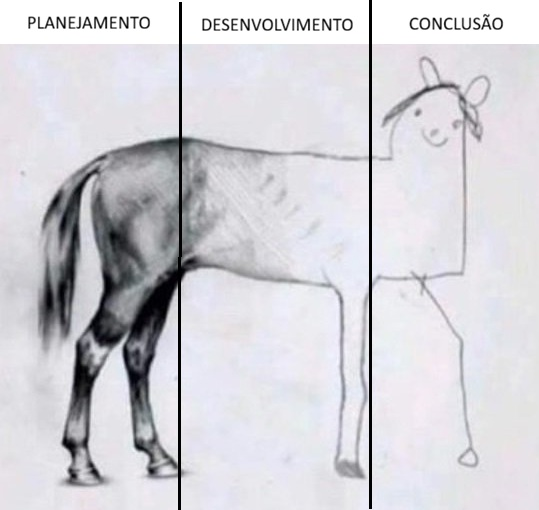
\includegraphics[keepaspectratio]{imagens/pesquisa_cientifica.jpg}}

}

\caption{\label{fig-pesquisa}Etapas do desenvolvimento da pesquisa
científica.}

\end{figure}%

\subsection*{Tables}\label{tables}
\addcontentsline{toc}{subsection}{Tables}

\pagebreak
\newpage

\section*{Apendices}\label{apendices}
\addcontentsline{toc}{section}{Apendices}

\section*{Non-used figures and
tables}\label{non-used-figures-and-tables}
\addcontentsline{toc}{section}{Non-used figures and tables}

\begin{tcolorbox}[enhanced jigsaw, title=\textcolor{quarto-callout-warning-color}{\faExclamationTriangle}\hspace{0.5em}{Non-used codes}, leftrule=.75mm, opacitybacktitle=0.6, colframe=quarto-callout-warning-color-frame, colback=white, titlerule=0mm, arc=.35mm, opacityback=0, left=2mm, bottomtitle=1mm, breakable, colbacktitle=quarto-callout-warning-color!10!white, coltitle=black, rightrule=.15mm, bottomrule=.15mm, toptitle=1mm, toprule=.15mm]

\end{tcolorbox}




\end{document}
